\section{Results}
\label{sec:results}

\subsection{Wave drag at short lengths}

Table~\ref{tab:cfd} gives the new direct Euler values. At $L/D = 3.5$ the report-1 interpolation
between $L/D = 3$ and 4 is within 0.6\,\% at $M = 1.4$ and 0.8\,\% at $M = 1.2$--1.6, so the
numbers quoted from it earlier hold. Below $L/D = 3$ report~1 had no data and held $C_{D,\rm w}(L/D)^2$
constant; the new runs show that this product keeps falling as the nose gets blunter, so the
extrapolation overestimated the wave drag of the shortest noses by 6--10\,\%. All results below use
the new data. The $M = 1.1$ runs, and the $M = 1.2$ runs of LV-Haack and power~$\tfrac12$ at
$L/D=2.5$, stopped at the 6000-iteration limit with a residual uncertainty of 1--2\,\%, as the
$M = 1.1$ runs of report~1.

\begin{table}[H]
\centering
\caption{Direct Euler wave drag $C_{D,\rm w}$ (sharp apex) and the error of the report-1 model
(interpolation at $L/D = 3.5$, extrapolation from $L/D = 3$ at 2.5).}
\label{tab:cfd}
\small
\begin{tabular}{@{}llrrrrr@{}}
\toprule
Profile & $L/D$ & $M=1.1$ & $M=1.2$ & $M=1.4$ & $M=1.6$ & report-1 model at $M=1.4$ \\
\midrule
Von K\'arm\'an & 2.5 & 0.1156 & 0.1212 & 0.1190 & 0.1155 & $+$5.7\,\% \\
Von K\'arm\'an & 3.5 & 0.0680 & 0.0686 & 0.0667 & 0.0648 & $-$0.4\,\% \\
LV-Haack & 2.5 & 0.1147 & 0.1302 & 0.1356 & 0.1347 & $+$7.1\,\% \\
LV-Haack & 3.5 & 0.0714 & 0.0767 & 0.0776 & 0.0766 & $-$0.6\,\% \\
Power $\tfrac12$ & 2.5 & 0.1052 & 0.1100 & 0.1122 & 0.1119 & $+$9.8\,\% \\
Power $\tfrac12$ & 3.5 & 0.0641 & 0.0665 & 0.0677 & 0.0675 & $-$0.5\,\% \\
\bottomrule
\end{tabular}

\end{table}

\subsection{Coupler length at 650 mm}

\begin{figure}[H]
\centering
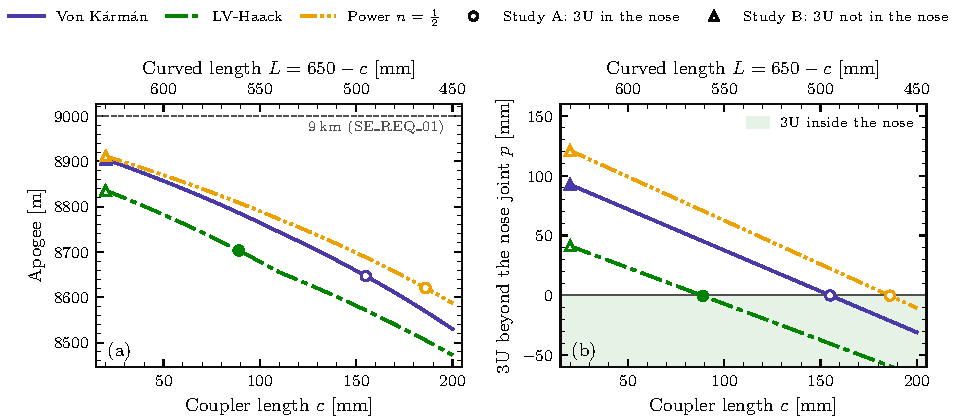
\includegraphics[width=\textwidth]{fig_tl_coupler}
\caption{Total length \SI{650}{mm}. (a) Apogee and (b) length of 3U past the nose joint against
the coupler length $c$. Markers: design point of each profile in study~A (circles) and B
(triangles); filled: the design chosen in each study.}
\label{fig:coupler}
\end{figure}

Figure~\ref{fig:coupler}a shows the cost of the coupler: the apogee falls by \SIrange{1.3}{1.7}{m}
per millimetre of coupler at $c = \TLCMIN$ and by about \SI{2}{m} per millimetre at
$c = \SIrange{100}{150}{mm}$, because the curved part gets shorter and blunter. At
equal length Von K\'arm\'an and power~$\tfrac12$ fly within \TLEQGAPPH{} of each other (the
difference is inside the model uncertainty), and \TLEQGAP{} higher than LV-Haack, as in report~1.

Figure~\ref{fig:coupler}b shows why this ranking does not decide study~A. With the shortest
coupler the 3U reaches \TLOutVKP{} (Von K\'arm\'an) and \TLOutPHP{} (power~$\tfrac12$) past the
joint, and each millimetre of coupler pulls it back by only $1-\kappa$ of a millimetre
(Equation~\ref{eq:p}). LV-Haack has the largest $\kappa$, so its curve starts lowest and reaches
zero first.

\subsection{Design points}

\begin{table}[H]
\centering
\caption{Design point of each profile in each study at \SI{650}{mm}. ``3U in $L$'': length of the
curved part with $r\geq\SI{77}{mm}$; $p$: 3U past the joint (in study~B, where it would reach if it
were in the nose). Bold: best, or within \SI{10}{m} of the best.}
\label{tab:designs}
\small
\begin{tabular}{@{}llrrrrrrr@{}}
\toprule
Study & Profile & $c$ & $L$ & $L/D$ & 3U in $L$ & $p$ & Apogee & vs \SI{9}{km} \\
 & & [mm] & [mm] & & [mm] & [mm] & [m] & [m] \\
\midrule
A: 3U in the nose & Von K\'arm\'an & 155 & 495 & 2.75 & 155 & 0 & 8647 & $-$353 \\
 & \textbf{LV-Haack} & 89 & 561 & 3.12 & 222 & $-$1 & \textbf{8703} & \textbf{$-$297} \\
 & Power $\tfrac12$ & 186 & 464 & 2.58 & 124 & 0 & 8621 & $-$379 \\
\midrule
B: 3U not in the nose & \textbf{Von K\'arm\'an} & 20 & 630 & 3.50 & 197 & 93 & \textbf{8905} & \textbf{$-$95} \\
 & LV-Haack & 20 & 630 & 3.50 & 249 & 41 & 8836 & $-$164 \\
 & \textbf{Power $\tfrac12$} & 20 & 630 & 3.50 & 169 & 121 & \textbf{8911} & \textbf{$-$89} \\
\bottomrule
\end{tabular}

\end{table}

\begin{itemize}[leftmargin=*,itemsep=2pt]
\item \textbf{Study A, 3U in the nose}: LV-Haack, \TLInLVHL{} curved + \TLInLVHC{} coupler,
\TLInLVHD. Von K\'arm\'an needs a \TLInVKC{} coupler, which leaves it only $L/D = \TLInVKLD$, and
loses \TLGAPVK; power~$\tfrac12$ loses \TLGAPPH. If the cylinder may instead be extended beyond
\SI{650}{mm}, keeping a \SI{630}{mm} curved part is not the best use of the extra length: Von
K\'arm\'an 630 + \SI{113}{mm} (\SI{743}{mm}) reaches \SI{8870}{m}, LV-Haack at \SI{740}{mm} in
total \SI{8906}{m} (Section~\ref{sec:length}).
\item \textbf{Study B, 3U not in the nose}: Von K\'arm\'an, \TLOutVKL{} curved + \TLOutVKC{}
coupler, \TLOutVKD; power~$\tfrac12$ (\TLOutPHD) is equal within the model uncertainty, but meets the
cylinder at an angle and is blunt at the tip. The 3U would reach \TLOutVKP{} past the joint, more
than the \SI{50}{mm} free in the RE tube (RE\_REQ\_08), so it has to go elsewhere. Moving it
\SI{100}{mm} aft moves the burn-out centre of gravity aft by about \TLGRVSM~cal, which SE and FD
have to include in the stability budget.
\item \textbf{A against B}: \TLAB{} at \SI{650}{mm}, the apogee of \TLABKG{} of dry mass.
\end{itemize}

\subsection{What a longer nose buys}
\label{sec:length}

\begin{figure}[H]
\centering
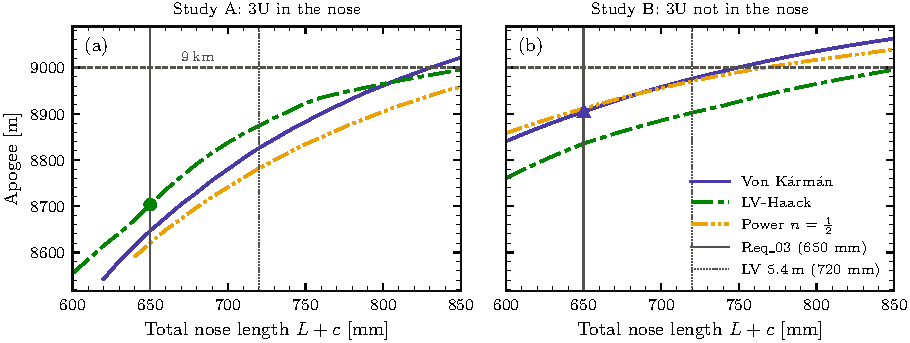
\includegraphics[width=\textwidth]{fig_tl_total}
\caption{Apogee against the allowed total length of the nose, each profile with the coupler of its
study. Solid vertical line: Req\_03; dotted: LV length \SI{5.4}{m} (SE\_REQ\_04) with the rest of
the LVO unchanged. Markers: the designs of Table~\ref{tab:final}.}
\label{fig:total}
\end{figure}

\begin{table}[H]
\centering
\caption{Best design at each allowed total length for the interface meeting (VK Von K\'arm\'an,
LVH LV-Haack; $L + c$ in mm; within \SI{10}{m}, Von K\'arm\'an is listed). Gain against the same
study at \SI{650}{mm}. LV: launch vehicle length with the rest of the LVO unchanged (italic: not
shorter than the \SI{5.4}{m} of SE\_REQ\_04).}
\label{tab:length}
\small
\begin{tabular}{@{}rrlrrlrr@{}}
\toprule
Total & LV & \multicolumn{3}{c}{Study A: 3U in the nose} & \multicolumn{3}{c}{Study B: 3U not in the nose} \\
\cmidrule(lr){3-5}\cmidrule(l){6-8}
$L+c$ [mm] & [m] & Design $L+c$ & Apogee [m] & Gain [m] & Design $L+c$ & Apogee [m] & Gain [m] \\
\midrule
650 & 5.33 & LVH 561\,+\,89 & 8703 & -- & VK 630\,+\,20 & 8905 & -- \\
700 & 5.38 & LVH 644\,+\,56 & 8837 & $+$134 & VK 680\,+\,20 & 8958 & $+$53 \\
720 & \textit{5.40} & LVH 677\,+\,43 & 8874 & $+$171 & VK 700\,+\,20 & 8976 & $+$71 \\
750 & \textit{5.43} & LVH 727\,+\,23 & 8923 & $+$219 & VK 730\,+\,20 & 9000 & $+$96 \\
800 & \textit{5.48} & VK 713\,+\,87 & 8961 & $+$257 & VK 780\,+\,20 & 9035 & $+$131 \\
850 & \textit{5.53} & VK 786\,+\,64 & 9021 & $+$318 & VK 830\,+\,20 & 9063 & $+$158 \\
\midrule
\multicolumn{2}{@{}l}{\SI{9}{km} reached at} & \multicolumn{3}{l}{$L+c\approx\SI{830}{mm}$ (LV \SI{5.51}{m})} & \multicolumn{3}{l}{$L+c\approx\SI{750}{mm}$ (LV \SI{5.43}{m})} \\
\bottomrule
\end{tabular}

\end{table}

Near \SI{650}{mm} each millimetre of allowed length is worth \TLInSLOPE{} in study~A and
\TLOutSLOPE{} in study~B (Figure~\ref{fig:total}, Table~\ref{tab:length}). In A the extra length
goes into the curved part, which also makes room for the 3U and lets the cylinder shrink: that is
why the gain is larger. LV-Haack stays the best choice in A up to about \SI{800}{mm}; beyond that the
3U fits in a long Von K\'arm\'an nose, which then wins. \SI{9}{km} needs about \TLInNINE{} in A and
\TLOutNINE{} in B, both beyond the \TLLVNOSE{} at which the LV reaches \SI{5.4}{m}. Within that cap
the nose is worth \TLInSEVENTWENTYG{} (A) and \TLOutSEVENTWENTYG{} (B); the rest of the shortfall
has to come from the vehicle (mass, drag, engine) or from a longer LV.

\subsection{Sensitivity}
\label{sec:sens}

\begin{itemize}[leftmargin=*,itemsep=2pt]
\item \textbf{Payload length} (study~A). With a \SI{340.5}{mm} 3U CubeSat instead of the
\SI{300}{mm} GRV, the coupler becomes \TLSENSLVHC{} with LV-Haack (\TLSENSLVHD), \TLSENSVKC{} with
Von K\'arm\'an (\TLSENSVKD) and \TLSENSPHC{} with power~$\tfrac12$ (\TLSENSPHD, extrapolated below
$L/D=2.5$). The ranking is unchanged; every \SI{10}{mm} of payload costs \SI{33}{m} with LV-Haack
and \SIrange{41}{45}{m} with the other two.
\item \textbf{Model.} A 1\,\% error on the wave drag moves the apogee of these noses by \SI{5}{m}
(study~B) to \SI{7}{m} (study~A). The \TLGAPVK{} margin of LV-Haack in study~A would therefore need
an error of about 9\,\% between two profiles, against the 0.5--1\,\% accuracy of the solver; it comes from the
geometry of the 3U fit, not from small drag differences. The absolute apogee depends on the drag
factor $k$, calibrated on the LVO, exactly as in report~1; the differences between the studies and
lengths do not.
\end{itemize}
